GenericLibrary, henceforth abbreviated to GL, is a DSL for
descriptions of GRACeFUL concept map components embedded in the
Haskell programming language.
%
The DSL addresses the issue of bridging the gap between constraint
programming and the visualisation layer by providing abstractions for
modular constraint programming.
%
These abstractions are targeted at simplifying the description of
GRACeFUL concept maps.

The DSL is divided into two parts.
%
The first part, \texttt{GCM}, allows the user to describe the
interactions of GRACeFUL concept map components and has facilities for
constructing new components from existing ones.
%
The second part, \texttt{CP}, features primitives for constructing
constraint programs which describe the behaviour of an individual
component.

\subsection{The language}

The GCM language describes components and how they are connected.
%
The core abstraction in GL is that of the \texttt{Port}.
%
A port is an entity which represents the way two components interact,
it generalises the way factors from \cite{D4.1} can interact with each
other.
%
Ports can also be viwed as an abstraction of the concept of constraint
variables from CFP.
%
Each component exposes some information about the system through
ports.
%
As an example, a pump component may present one port for the current
flow of water being pumped and another port for the maximum flow of
the pump.

We first show the code for a somewhat simpler example: a \texttt{GCM}
component modelling a fixed amount of rain falling from the sky.
\begin{verbatim}
rain :: Float -> GCM (Port Float)
rain amount = do
  port <- createPort
  set port amount
  return port
\end{verbatim}

The CP language supports reasoning about integer and floating-point
arithmetic, boolean expressions, and arrays.
%
It has constructions like \texttt{value}, which reads the value from a
port, and \texttt{assert} for expression constraints on the behaviour
of a component.
%
Computations in \texttt{CP} can be embedded in \texttt{GCM} using the
\texttt{component} primitive.

We can now return to our pump, which is a \texttt{GCM} component
parameterised over the maximum flow through the pump:
%
\begin{verbatim}
pump :: Float -> GCM (Port Float, Port Float)
pump maxCap = do
  inPort  <- createPort
  outPort <- createPort
  component $ do             -- This is in CP
    inflow  <- value inPort
    outflow <- value outPort
    assert $  inflow === outflow
    assert $  inflow `inRange` (0, lit maxCap)
  return (inPort, outPort)
\end{verbatim}
%
Note that we need to use \texttt{lit} to lift \texttt{maxCap}, which
is a value in the host language Haskell, into the embeddedd langauge
GL.

Finally we show a more complicated component, a water storage with
an \texttt{inflow}, an \texttt{outlet} to which we may connect e.g. a pump,
and an \texttt{overflow}.
\begin{verbatim}
storage :: Float -> GCM (Port Float, Port Float, Port Float)
storage cap = do
  inflow   <- createPort
  outlet   <- createPort
  overflow <- createPort
  component $ do
    currentStored <- createVariable
    inf <- value inflow
    out <- value outlet
    ovf <- value overflow
    sto <- value currentStored
    assert $ sto === inf - out - ovf
    assert $ sto `inRange` (0, lit cap)
    assert $ (ovf .> 0) ==> (sto === lit cap)
    assert $ ovf .>= 0
  return (inflow, outlet, overflow)
\end{verbatim}

In conclusion, we have seen that there is a clear separation of concerns in GL between
the high level primitives for constructing complicated components from
simpler ones, expressed in \texttt{GCM}, and the low level
implementation details with which the \texttt{CP} language is
concerned.

\subsection{Expressing GRACeFUL concept map elements in GL}
Many of the elements of GRACeFUL concept maps identified in
\cite{D4.1} can be modeled in GL using language primitives such as
\texttt{linkBy} (for connections), \texttt{createAction} (for
actions), \texttt{assert} (for constraints) etc.
GL being an \textit{embedded} domain specific language featuring a
rich set of primitive operations for reasoning in the target domain
allows the programmer to construct abstractions which capture
behaviour which generalises many of the concepts described in
\cite{D4.1}.
%
\begin{wrapfigure}{r}{0.5\textwidth}
  \centering
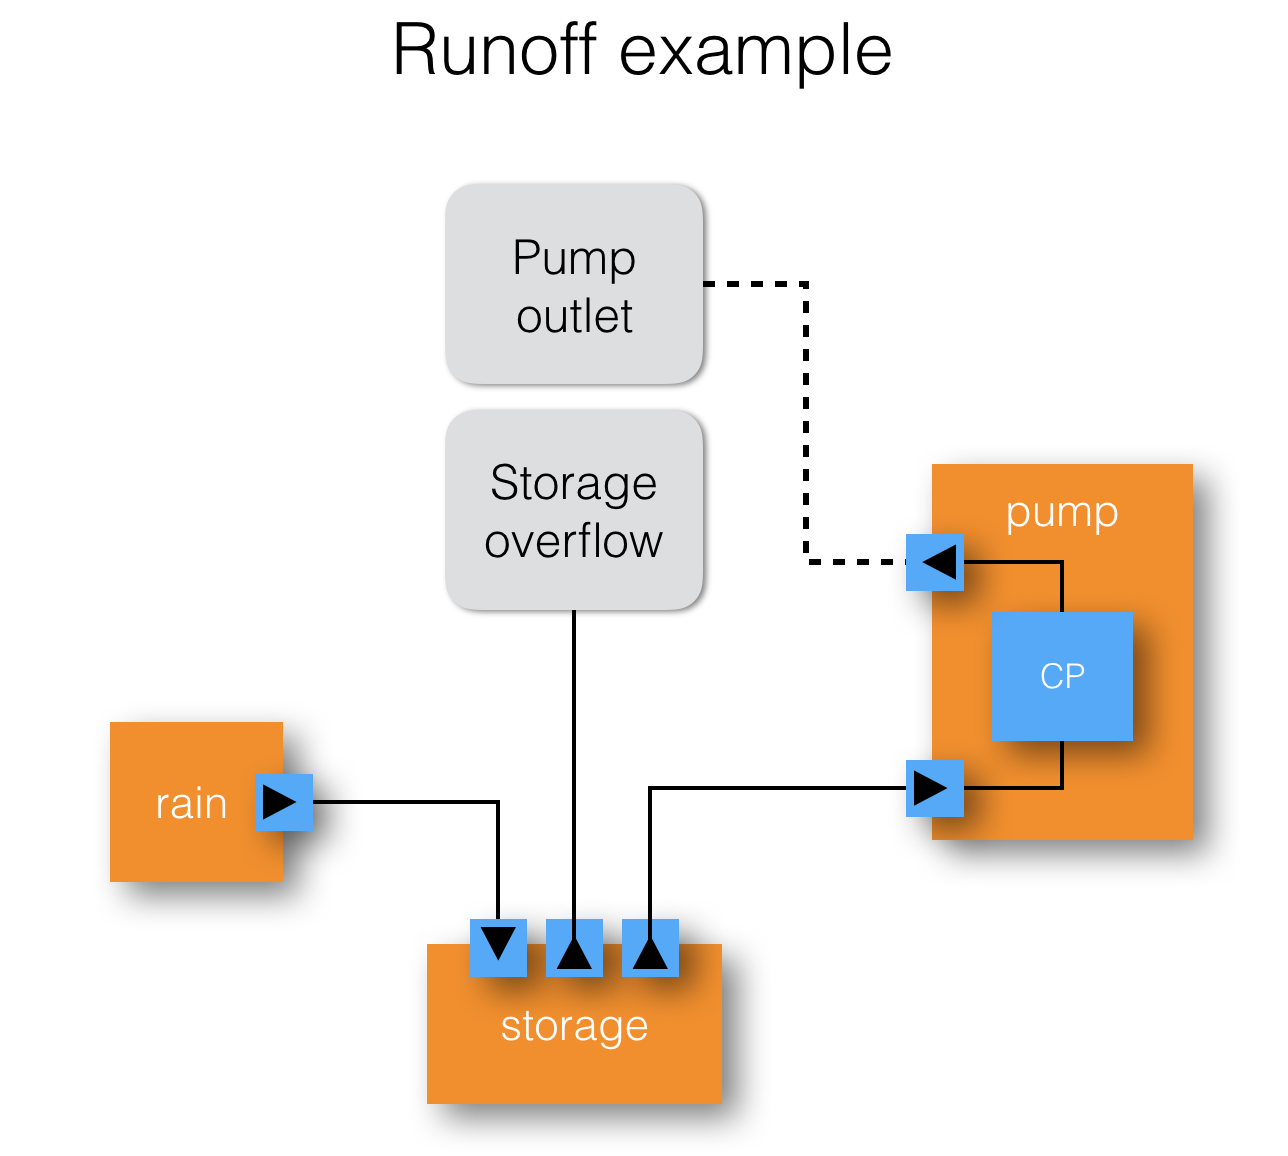
\includegraphics[width=0.48\textwidth]{fig/RunoffExample.jpg}
  \caption{Runoff example structure}
  \label{fig:RunoffEx}
\end{wrapfigure}
%
